\documentclass[a4paper]{article}
\usepackage[utf8]{inputenc}
\usepackage[spanish, es-tabla]{babel}
\usepackage{xcolor}
\usepackage{amsmath}
\usepackage{amsfonts}
\usepackage{amssymb}

\usepackage{float}
\usepackage{graphicx}
\graphicspath{ {./Imagenes/} }

\usepackage{multirow}
\setlength{\doublerulesep}{\arrayrulewidth}

\usepackage{tikz}
\usetikzlibrary{matrix,calc}

\usepackage{array}
\newcolumntype{C}[1]{>{\centering\let\newline\\\arraybackslash\hspace{0pt}}m{#1}}

\usepackage[american]{circuitikz}

\usepackage{fancyhdr}

\usepackage{units} 

\pagestyle{fancy}
\fancyhf{}
\lhead{22.13 Electrónica III}
\rhead{Mechoulam, Lambertucci, Martorell, Londero}
\rfoot{Página \thepage}

\newcommand{\quotes}[1]{``#1''}

\usepackage{tikz}
\usetikzlibrary{matrix,calc}

%isolated term
%#1 - Optional. Space between node and grouping line. Default=0
%#2 - node
%#3 - filling color
\newcommand{\implicantsol}[3][0]{
    \draw[rounded corners=3pt, fill=#3, opacity=0.3] ($(#2.north west)+(135:#1)$) rectangle ($(#2.south east)+(-45:#1)$);
    }


%internal group
%#1 - Optional. Space between node and grouping line. Default=0
%#2 - top left node
%#3 - bottom right node
%#4 - filling color
\newcommand{\implicant}[4][0]{
    \draw[rounded corners=3pt, fill=#4, opacity=0.3] ($(#2.north west)+(135:#1)$) rectangle ($(#3.south east)+(-45:#1)$);
    }

%group lateral borders
%#1 - Optional. Space between node and grouping line. Default=0
%#2 - top left node
%#3 - bottom right node
%#4 - filling color
\newcommand{\implicantcostats}[4][0]{
    \draw[rounded corners=3pt, fill=#4, opacity=0.3] ($(rf.east |- #2.north)+(90:#1)$)-| ($(#2.east)+(0:#1)$) |- ($(rf.east |- #3.south)+(-90:#1)$);
    \draw[rounded corners=3pt, fill=#4, opacity=0.3] ($(cf.west |- #2.north)+(90:#1)$) -| ($(#3.west)+(180:#1)$) |- ($(cf.west |- #3.south)+(-90:#1)$);
}

%group top-bottom borders
%#1 - Optional. Space between node and grouping line. Default=0
%#2 - top left node
%#3 - bottom right node
%#4 - filling color
\newcommand{\implicantdaltbaix}[4][0]{
    \draw[rounded corners=3pt, fill=#4, opacity=0.3] ($(cf.south -| #2.west)+(180:#1)$) |- ($(#2.south)+(-90:#1)$) -| ($(cf.south -| #3.east)+(0:#1)$);
    \draw[rounded corners=3pt, fill=#4, opacity=0.3] ($(rf.north -| #2.west)+(180:#1)$) |- ($(#3.north)+(90:#1)$) -| ($(rf.north -| #3.east)+(0:#1)$);
}

%group corners
%#1 - Optional. Space between node and grouping line. Default=0
%#2 - filling color
\newcommand{\implicantcantons}[2][0]{
    \draw[rounded corners=3pt, opacity=.3] ($(rf.east |- 0.south)+(-90:#1)$) -| ($(0.east |- cf.south)+(0:#1)$);
    \draw[rounded corners=3pt, opacity=.3] ($(rf.east |- 8.north)+(90:#1)$) -| ($(8.east |- rf.north)+(0:#1)$);
    \draw[rounded corners=3pt, opacity=.3] ($(cf.west |- 2.south)+(-90:#1)$) -| ($(2.west |- cf.south)+(180:#1)$);
    \draw[rounded corners=3pt, opacity=.3] ($(cf.west |- 10.north)+(90:#1)$) -| ($(10.west |- rf.north)+(180:#1)$);
    \fill[rounded corners=3pt, fill=#2, opacity=.3] ($(rf.east |- 0.south)+(-90:#1)$) -|  ($(0.east |- cf.south)+(0:#1)$) [sharp corners] ($(rf.east |- 0.south)+(-90:#1)$) |-  ($(0.east |- cf.south)+(0:#1)$) ;
    \fill[rounded corners=3pt, fill=#2, opacity=.3] ($(rf.east |- 8.north)+(90:#1)$) -| ($(8.east |- rf.north)+(0:#1)$) [sharp corners] ($(rf.east |- 8.north)+(90:#1)$) |- ($(8.east |- rf.north)+(0:#1)$) ;
    \fill[rounded corners=3pt, fill=#2, opacity=.3] ($(cf.west |- 2.south)+(-90:#1)$) -| ($(2.west |- cf.south)+(180:#1)$) [sharp corners]($(cf.west |- 2.south)+(-90:#1)$) |- ($(2.west |- cf.south)+(180:#1)$) ;
    \fill[rounded corners=3pt, fill=#2, opacity=.3] ($(cf.west |- 10.north)+(90:#1)$) -| ($(10.west |- rf.north)+(180:#1)$) [sharp corners] ($(cf.west |- 10.north)+(90:#1)$) |- ($(10.west |- rf.north)+(180:#1)$) ;
}

%Empty Karnaugh map 4x4
\newenvironment{Karnaugh}%
{
\begin{tikzpicture}[baseline=(current bounding box.north),scale=0.8]
\draw (0,0) grid (4,4);
\draw (0,4) -- node [pos=0.7,above right,anchor=south west] {ba} node [pos=0.7,below left,anchor=north east] {dc} ++(135:1);
%
\matrix (mapa) [matrix of nodes,
        column sep={0.8cm,between origins},
        row sep={0.8cm,between origins},
        every node/.style={minimum size=0.3mm},
        anchor=8.center,
        ampersand replacement=\&] at (0.5,0.5)
{
                       \& |(c00)| 00         \& |(c01)| 01         \& |(c11)| 11         \& |(c10)| 10         \& |(cf)| \phantom{00} \\
|(r00)| 00             \& |(0)|  \phantom{0} \& |(1)|  \phantom{0} \& |(3)|  \phantom{0} \& |(2)|  \phantom{0} \&                     \\
|(r01)| 01             \& |(4)|  \phantom{0} \& |(5)|  \phantom{0} \& |(7)|  \phantom{0} \& |(6)|  \phantom{0} \&                     \\
|(r11)| 11             \& |(12)| \phantom{0} \& |(13)| \phantom{0} \& |(15)| \phantom{0} \& |(14)| \phantom{0} \&                     \\
|(r10)| 10             \& |(8)|  \phantom{0} \& |(9)|  \phantom{0} \& |(11)| \phantom{0} \& |(10)| \phantom{0} \&                     \\
|(rf) | \phantom{00}   \&                    \&                    \&                    \&                    \&                     \\
};
}%
{
\end{tikzpicture}
}

%Empty Karnaugh map 2x4
\newenvironment{Karnaughvuit}%
{
\begin{tikzpicture}[baseline=(current bounding box.north),scale=0.8]
\draw (0,0) grid (4,2);
\draw (0,2) -- node [pos=0.7,above right,anchor=south west] {bc} node [pos=0.7,below left,anchor=north east] {a} ++(135:1);
%
\matrix (mapa) [matrix of nodes,
        column sep={0.8cm,between origins},
        row sep={0.8cm,between origins},
        every node/.style={minimum size=0.3mm},
        anchor=4.center,
        ampersand replacement=\&] at (0.5,0.5)
{
                      \& |(c00)| 00         \& |(c01)| 01         \& |(c11)| 11         \& |(c10)| 10         \& |(cf)| \phantom{00} \\
|(r00)| 0             \& |(0)|  \phantom{0} \& |(1)|  \phantom{0} \& |(3)|  \phantom{0} \& |(2)|  \phantom{0} \&                     \\
|(r01)| 1             \& |(4)|  \phantom{0} \& |(5)|  \phantom{0} \& |(7)|  \phantom{0} \& |(6)|  \phantom{0} \&                     \\
|(rf) | \phantom{00}  \&                    \&                    \&                    \&                    \&                     \\
};
}%
{
\end{tikzpicture}
}

%Empty Karnaugh map 2x2
\newenvironment{Karnaughquatre}%
{
\begin{tikzpicture}[baseline=(current bounding box.north),scale=0.8]
\draw (0,0) grid (2,2);
\draw (0,2) -- node [pos=0.7,above right,anchor=south west] {b} node [pos=0.7,below left,anchor=north east] {a} ++(135:1);
%
\matrix (mapa) [matrix of nodes,
        column sep={0.8cm,between origins},
        row sep={0.8cm,between origins},
        every node/.style={minimum size=0.3mm},
        anchor=2.center,
        ampersand replacement=\&] at (0.5,0.5)
{
          \& |(c00)| 0          \& |(c01)| 1  \\
|(r00)| 0 \& |(0)|  \phantom{0} \& |(1)|  \phantom{0} \\
|(r01)| 1 \& |(2)|  \phantom{0} \& |(3)|  \phantom{0} \\
};
}%
{
\end{tikzpicture}
}

%Defines 8 or 16 values (0,1,X)
\newcommand{\contingut}[1]{%
\foreach \x [count=\xi from 0]  in {#1}
     \path (\xi) node {\x};
}

%Places 1 in listed positions
\newcommand{\minterms}[1]{%
    \foreach \x in {#1}
        \path (\x) node {1};
}

%Places 0 in listed positions
\newcommand{\maxterms}[1]{%
    \foreach \x in {#1}
        \path (\x) node {0};
}

%Places X in listed positions
\newcommand{\indeterminats}[1]{%
    \foreach \x in {#1}
        \path (\x) node {X};
}

% \begin{document}
%     \begin{Karnaugh}
%         \contingut{0,0,0,0,0,0,0,0,0,0,0,0,0,0,0,0}
%        \implicant{0}{2}{red}
%        \implicant{5}{15}{purple}
%        \implicantdaltbaix[3pt]{3}{10}{blue}
%     \implicantcantons[2pt]{orange}
%        \implicantcostats{4}{14}{green}
%     \end{Karnaugh}
%     %
%     \begin{Karnaughvuit}
%        \minterms{3,4}
%         \maxterms{0,1,6,7}
%        \indeterminats{2,5}
%        \implicant{3}{2}{green}
%        \implicant{4}{5}{}
%     \end{Karnaughvuit}
%     %
%     \begin{Karnaughquatre}
%         \minterms{1,2}
%        \maxterms{0,3}
%        \implicantsol{1}{green}
%        \implicantsol{2}{red}
%     \end{Karnaughquatre}

% \end{document}

\begin{document}

%%%%%%%%%%%%%%%%%%%%%%%%%%%%%%%%%%%%%%%%%%%%%%%%%%%%%%%%%%%%%%%%%%%%%%%%% 
%								CARATULA								%
%%%%%%%%%%%%%%%%%%%%%%%%%%%%%%%%%%%%%%%%%%%%%%%%%%%%%%%%%%%%%%%%%%%%%%%%% 

\begin{titlepage}
\newcommand{\HRule}{\rule{\linewidth}{0.5mm}}
\center
\mbox{\textsc{\LARGE \bfseries {Instituto Tecnológico de Buenos Aires}}}\\[1.5cm]
\textsc{\Large 22.13 Electrónica III}\\[0.5cm]


\HRule \\[0.6cm]
{ \Huge \bfseries Trabajo práctico N$^{\circ}$1}\\[0.4cm] 
\HRule \\[1.5cm]


{\large

\emph{Grupo 3}\\
\vspace{3px}

\begin{tabular}{lr} 	
\textsc{Mechoulam}, Alan  &  58438\\
\textsc{Lambertucci}, Guido Enrique  & 58009 \\
\textsc{Martorell}, Ariel  & 56209 \\
\textsc{Londero Bonaparte}, Tomás Guillermo  & 58150 \\
\end{tabular}

\vspace{20px}

\emph{Profesor}\\
\vspace{3px}
\textsc{Dewald}, Kevin\\	

\vspace{100px}

\begin{tabular}{ll}

Presentado: & /19\\

\end{tabular}

}

\vfill

\end{titlepage}


%%%%%%%%%%%%%%%%%%%%%%%%%%%%%%%%%%%%%%%%%%%%%%%%%%%%%%%%%%%%%%%%%%%%%%%%% 
%								INFORME									%
%%%%%%%%%%%%%%%%%%%%%%%%%%%%%%%%%%%%%%%%%%%%%%%%%%%%%%%%%%%%%%%%%%%%%%%%%

\section*{Introducción}


\section*{Desarrollo de la experiencia}

\subsection*{Ejercicio 1}
\subsubsection*{Introducción}
Se realizo un programa que calcula el rango y resolución de una convención dada de punto fijo. Se le debe pasar a este tres parámetros en el orden que se presenta a continuación:
\begin{itemize}
\item Un 1 si se considera al numero signado o un 0 si se lo considera no signado.
\item Cantidad de bits de la parte entera.
\item Cantidad de bits de la parte fraccionaria.
\end{itemize}

Ante cualquier entrada que sea considerada como un error, se imprime un mensaje de \quotes{ERROR} por consola. Ante una entrada válida, imprime el rango y resolución calculado.

\subsubsection*{Consideraciones}

A continuación se detallan las consideraciones tomadas junto al análisis realizado de cada caso:
\begin{itemize}
\item \textbf{Argumento faltante:} Se consideró como un error la falta de un argumento por más que se pueda optar por igualar al faltante a cero, ya que las instrucciones dentro del archivo son claras.
\item \textbf{Agumento adicional:} No se podría realizar nada con un argumento adicional por lo que se lo consideró como un error.
\item \textbf{Limitaciones al primer argumento:} El primer argumento adjudica si el programa considerará la convención signada o no signada, por esta razón puede tomar sólamente dos valores, 1 o 0. Cualquier otro valor será un error.
\item \textbf{Límite inferior de argumento:} Se consideró por fijar un límite inferior a los argumentos igual a 0, ya que valores negativos carecían de sentido.
\item \textbf{Límite superior de argumento:} Por más que incluyendo ciertos paquetes de python al script, la posibilidad de tener números muy pequeños o muy grandes esta limitado por la cantidad de memoria disponible, se optó por fijar un límite superior ya que el exponente del número normalizado más grande (o más pequeño, siendo el exponente negativo) es de 308. Por esta razón se eligió un límite superior de 1023 ya que $2^{1023} \approx 9\cdot 10^{307}$.
\item \textbf{Argumento no numérico:} No se realizó ningún tipo de conversión de letra a número, por lo que se consideró error cualquier entrada no numérica.

\end{itemize}

\subsection*{Ejercicio 2}

Dadas las siguientes expresiones:

\begin{equation}
f \left( e,d,c,b,a \right) = \sum m \left( 0,2,4,7,8,10,12,16,18,20,23,24,25,26,27,28 \right)
\label{equ:minterms}
\end{equation}

\begin{equation}
f \left( d,c,b,a \right) = \prod \left( M_0,M_2,M_4,M_7,M_8,M_{10},M_{12} \right)
\label{equ:maxterms}
\end{equation}
se procede a hallar la mínima expresión posible para ambas, usando tanto álgebra booleana, como mapas de Karnaugh.
Escribiendo (\ref{equ:minterms}) en forma de minterminos se obtiene:
\begin{center}
\[
	f \left( e,d,c,b,a \right) = \bar{e}\bar{d}\bar{c}\bar{b}\bar{a} \ + \ \bar{e}\bar{d}\bar{c}b\bar{a} \ + \ \bar{e}\bar{d}c\bar{b}\bar{a} \ + \ \bar{e}\bar{d}cba \ + \ \bar{e}d\bar{c}\bar{b}\bar{a} \ + \ \bar{e}d\bar{c}b\bar{a} \ + \ \bar{e}dc\bar{b}\bar{a} \ +
\]
\[
	e\bar{d}\bar{c}\bar{b}\bar{a} \ + \ e\bar{d}\bar{c}b\bar{a} \ + \ e\bar{d}c\bar{b}\bar{a} \ + \ e\bar{d}cba \ + \ ed\bar{c}\bar{b}\bar{a}\ + \ ed\bar{c}\bar{b}a \ + \ ed\bar{c}b\bar{a} \ + \ ed\bar{c}ba \ + \ edc\bar{b}\bar{a} 
\]

Su desarrollo utilizando álgebra booleana es el siguiente:
\[
	f \left( e,d,c,b,a \right) = \underbrace{\bar{e}\bar{d}\bar{c}\bar{b}\bar{a} \ + \ \bar{e}\bar{d}\bar{c}b\bar{a} }_{\bar{e}\bar{d}\bar{c}\bar{a}}\ + 							\underbrace{\bar{e}\bar{d}\bar{c}\bar{b}\bar{a} \ + \bar{e}\bar{d}c\bar{b}  \bar{a}  }_{\bar{e}\bar{d}\bar{b}\bar{a}}\  +
				\underbrace{\bar{e}\bar{d} c \bar{b}\bar{a} \ + e \bar{d} c\bar{b}  \bar{a}  }_{\bar{d}c\bar{b}\bar{a}}\  +
				\underbrace{\bar{e}\bar{d} c b a \ + e \bar{d} c b a  }_{ \bar{d} c b a}\ +
\]
\[
				\underbrace{\bar{e} d  \bar{c} \bar{b} \bar{a} \ + \bar{e} d \bar{c} b \bar{a}  }_{ \bar{e} d \bar{c}  \bar{a}}\ +
				\underbrace{\bar{e} d  c \bar{b} \bar{a} \ + \bar{e} d \bar{c} \bar{b} \bar{a}  }_{ \bar{e} d \bar{b}  \bar{a}}\ +
				\underbrace{\bar{e} d  c \bar{b} \bar{a} \ + e d c \bar{b} \bar{a}  }_{  d c \bar{b}  \bar{a}}\ +
				\underbrace{e \bar{d} \bar{c} \bar{b} \bar{a} \ + e \bar{d} \bar{c} b \bar{a}  }_{  e\bar{d}  \bar{c}  \bar{a}}\ +
\]
\[
				\underbrace{e d \bar{c} \bar{b} \bar{a} \ + e d \bar{c} \bar{b} a }_{  e d  \bar{c}  \bar{b}}\ +
				\underbrace{e  d \bar{c} \bar{b} a \ + e d \bar{c} b a  }_{  ed  \bar{c}  a}\ +
				\underbrace{\underbrace{e d \bar{c} \bar{b} \bar{a} \ + e d \bar{c} b \bar{a}  }_{  ed  \bar{c}  \bar{a}}\ +
				\underbrace{e d \bar{c} \bar{b} a \ + e d \bar{c} b a  }_{ ed \bar{c}  \bar{a}}}_{  ed  \bar{c}  \bar{a}} =
\]
De la anterior expresión, reordenando se consigue:
\[
				f \left( e,d,c,b,a \right) =\underbrace{\bar{e} \bar{d} \bar{c} \bar{b} \bar{a} \ + e \bar{d} \bar{c} \bar{a}  }_{  \bar{d}  \bar{c}  \bar{a}}\ +
						\underbrace{\bar{e} \bar{d} \bar{b} \bar{a}  \ + \bar{e} \bar{d} \bar{b} \bar{a}  }_{  \bar{d}  c b a}\ +
						\bar{d} cba + ed\bar{c}\bar{b}+
						\underbrace{\bar{d} c \bar{b} \bar{a} \ + d c \bar{b} \bar{a}  }_{  c \bar{b} \bar{a}}\ +
\]
\[	
					\underbrace{e d  \bar{c} \bar{a} \ + e d \bar{c} a  }_{  ed \bar{c} }\ +
					\underbrace{\bar{e} d \bar{c} \bar{a} \ + e d \bar{c} \bar{a}  }_{  d \bar{c} \bar{a}}
\]
\[	
				f \left( e,d,c,b,a \right) =\underbrace{\bar{d}   \bar{c} \bar{a} \ + d  \bar{c} \bar{a}   }_{  \bar{c}\bar{a} }\ +
						\underbrace{e  d \bar{c} \ +e d  \bar{c} \bar{b}   }_{  e  d \bar{c}  }\ +\bar{d}cba+\bar{e}\bar{b}\bar{a}+c\bar{b}\bar{a}
\]
teniendo en cuenta que 

\[
		c\bar{b}\bar{a}= ec\bar{b}\bar{a}+\bar{e}c\bar{b}\bar{a}+\bar{c}\bar{e}\bar{b}\bar{a}
\]
\[
		\bar{e}\bar{b}\bar{a}=c\bar{e}\bar{b}\bar{a}+\bar{c}\bar{e}\bar{b}\bar{a}+ce\bar{b}\bar{a}
\]
\[
	\underbrace{\underbrace{\bar{e}\bar{b}\bar{a} \ + ce\bar{b}\bar{a}  }_{ \bar{b}\bar{a}}\ 
	\underbrace{c\bar{b}\bar{a} \ + ce\bar{b}\bar{a}  }_{ \bar{b}\bar{a}}\ }_{\bar{b}\bar{a}}
\]
se llega a la expresión

\begin{equation}
		f \left( e,d,c,b,a \right) =bac\bar{d}+ed\bar{c}+\bar{c}\bar{a}+\bar{b}\bar{a}
		\label{equ:boolmin}
\end{equation}
\end{center}

Por otro lado, utilizando mapas de Karnaugh se consiguen los siguientes gráficos:

\begin{centering}
    \begin{Karnaugh}
        \minterms{0,2,4,7,8,10,12}
        \maxterms{1,3,5,6,9,11,13,14,15}
        
        \implicant{0}{8}{green}
        \implicantsol{7}{red}

        \implicantcantons{blue}
        
    \end{Karnaugh}
\par\end{centering}

\begin{center}
\textbf{e = 0}
\end{center}

\begin{centering}
    \begin{Karnaugh}
 \minterms{0,2,4,7,8,9,10,11,12}
        \maxterms{1,3,5,6,13,14,15}
        
        \implicant{0}{8}{green}
        \implicantsol{7}{red}
        \implicant{8}{10}{orange}

        \implicantcantons{blue}
        
    \end{Karnaugh}
\par\end{centering}

\begin{center}
\textbf{e = 1}
\end{center}

\begin{table}[H]
\centering
\caption{Mapa de Karnaugh de la expresión (\ref{equ:minterms}).}
\label{tabla:maxterms}
\end{table}



En este se pueden observar 4 grupos distintos:
\begin{enumerate}
	\item Compuesto por los casilleros 0, 4, 8, 12, 16, 20, 24 y 28, obteniéndose la expresión $ b a \bar{d} c $;
	\item Compuesto por los casilleros 7 y 23, obteniéndose la expresión $ e d \bar{c} $;
	\item Compuesto por los casilleros 0, 2, 8, 10, 16, 18, 24 y 26, obteniéndose la expresión $ \bar{c} \bar{a} $;
	\item Compuesto por los casilleros 24, 25, 26 y 27, obteniéndose la expresión $ \bar{b} \bar{a} $
\end{enumerate}

de esta forma se llega a la expresión:
\[
	f \left( e,d,c,b,a \right) = b a \bar{d} c \ + \  e d \bar{c} \ + \ \bar{c} \bar{a} \ + \ \bar{b} \bar{a}
\]
la cual coincide con (\ref{equ:boolmin}). De esta forma se representa, mediante un circuito de compuertas lógicas, la formula hallada.

\begin{figure}[H]
	\centering
	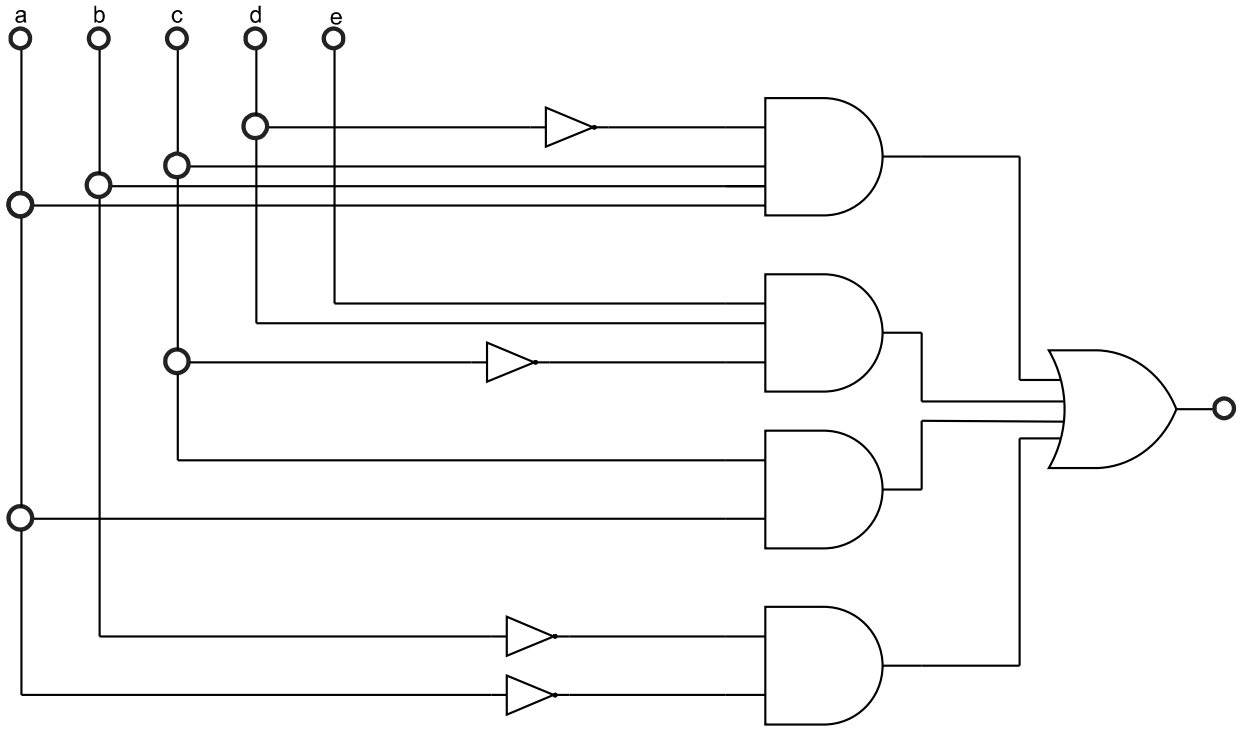
\includegraphics[width=0.9\textwidth]{Circuito1.PNG}
\caption{Circuito resultante de simplificar (\ref{equ:minterms}).}
	\label{fig:circ1}
\end{figure}

\begin{center}
Luego se dedujo una expresión para escribirlo con compuertas \textbf{NOR}.
\[
	f \left( e,d,c,b,a \right) = \overline{\overline{b a \bar{d} c }} \ + \  \overline{\overline{ e d \bar{c}}} \ + \ \overline{\overline{\bar{c} \bar{a}}} \ + \ \overline{\overline{ \bar{b} \bar{a}}}
\]
\[
	f \left( e,d,c,b,a \right) =\overline{\overline{\overline{\bar{b}+\bar{a}+d+\bar{c}}+\overline{\bar{e}+\bar{d}+c}+\overline{c+a}+\overline{b+a}}}
\]
Al desarrollo anterior le corresponde el siguiente circuito:
\begin{figure}[H]
	\hspace*{-1cm}
	\centering
	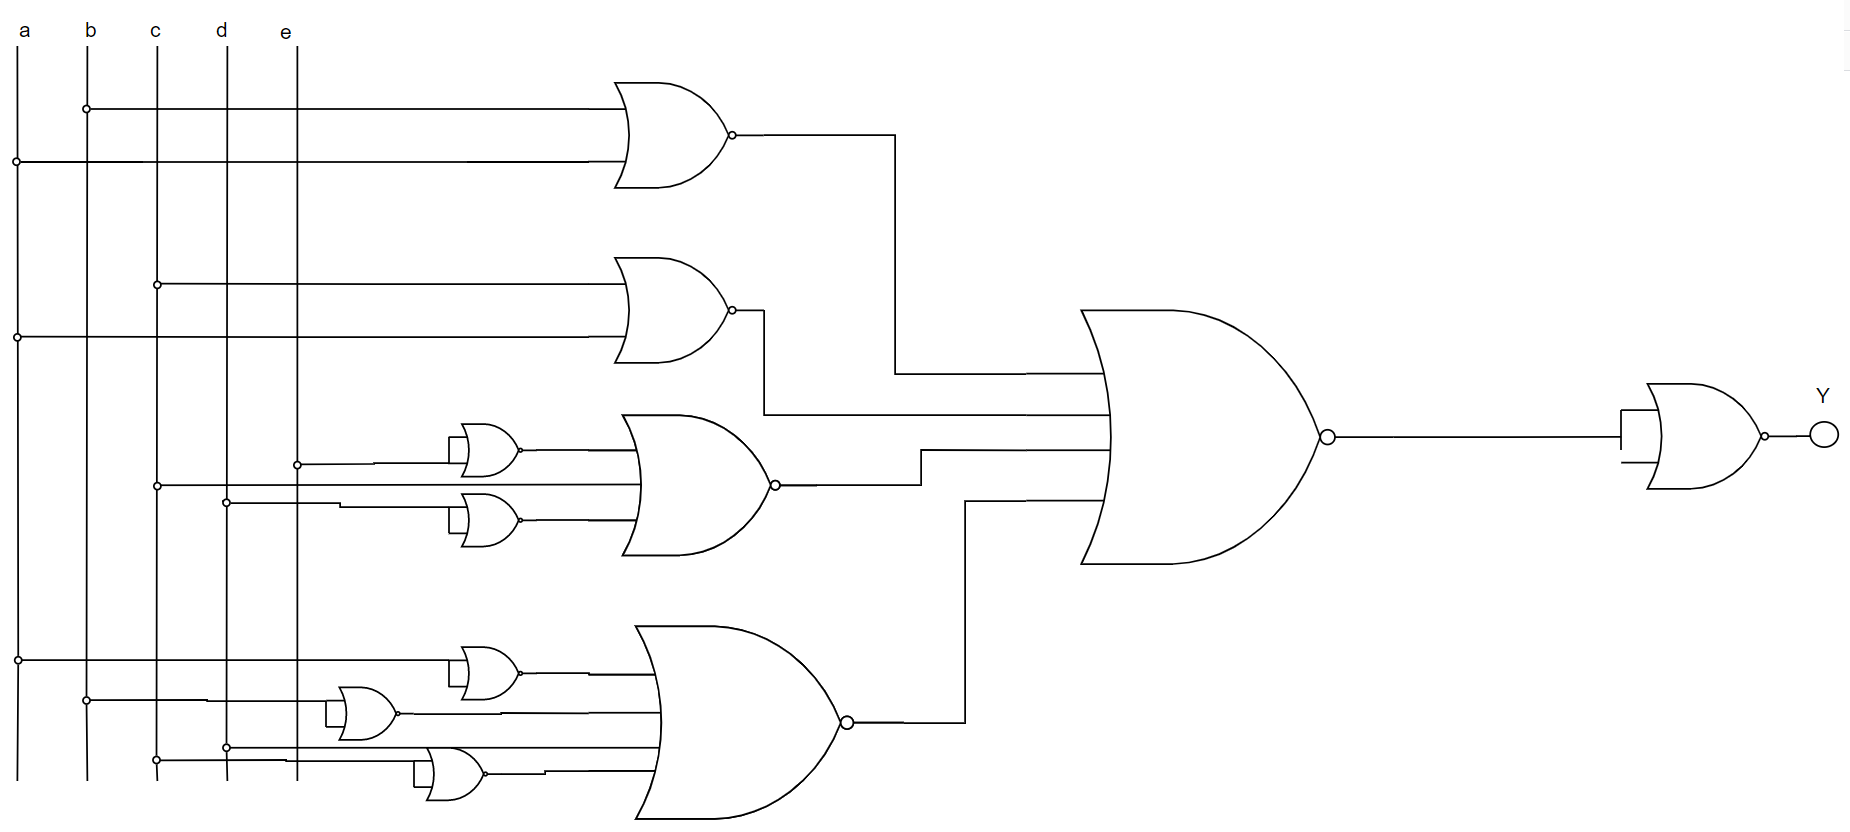
\includegraphics[width=1.2\textwidth]{Circuito4.png}
	\caption{Circuito unicamente con NOR.}
	\label{fig:circ4}
\end{figure}

Por otro lado, (\ref{equ:maxterms}) se escribe en forma de maxterminos:
\[
	f \left( d,c,b,a \right) = \left( a + b + c + d \right) \cdot \left( a + \bar{b} + c + d\right) \cdot \left( a + b+ \bar{c} + d \right) \cdot \left( \bar{a} + \bar{b} + \bar{c} + d \right) \cdot
\]
\[
	\left( a + b + c + \bar{d} \right) \cdot \left( a + \bar{b} + c + \bar{d} \right) \cdot \left( a + b + \bar{c} +\bar{d} \right)
\]

A su vez, esta puede ser expresada como
\[
	f \left( d,c,b,a \right) = a\bar{b}\bar{c}\bar{d} + ab\bar{c}\bar{d} +
	a\bar{b}c\bar{d} + a\bar{b}cd + a\bar{b}\bar{c}d + ab\bar{c}d + \bar{a}bc\bar{d} + \bar{a}bcd + abcd
\]

Su desarrollo utilizando álgebra booleana es el siguiente:
\[
	f \left( d,c,b,a \right) = \underbrace{a\bar{b}\bar{c}\bar{d} + ab\bar{c}\bar{d}}_{a\bar{c}\bar{d}} +
	\underbrace{a\bar{b}c\bar{d} + a\bar{b}cd}_{a\bar{b}c} + \underbrace{a\bar{b}\bar{c}d + ab\bar{c}d}_{a\bar{c}d} + \underbrace{\bar{a}bc\bar{d} + \bar{a}bcd}_{\bar{a}bc} + abcd
\]

\[
	f \left( d,c,b,a \right) = \bar{a}bc + \underbrace{a\bar{c}\bar{d} + a\bar{c}d}_{a\bar{c}} + a\bar{b}c + \underbrace{abcd + ab\bar{c}d}_{abd} + \underbrace{a\bar{b}\bar{c}\bar{d} + a\bar{b}\bar{c}d}_{a\bar{b}\bar{c}} 
\]

\[
	f \left( d,c,b,a \right) = a\bar{c} + \bar{a}bc + abd + \underbrace{a\bar{b}\bar{c} + a\bar{b}c}_{a\bar{b}}
\]

\[
	f \left( d,c,b,a \right) = a\bar{c} + \bar{a}bc + abd + a\bar{b} = a\bar{c} + \bar{a}bc + a \left( \bar{b} + bd \right) = a\bar{c} + \bar{a}bc + a \left( \bar{b} + d \right)
\]

Luego,
\begin{equation}
f \left( d,c,b,a \right) = a\bar{c} + \bar{a}bc + a\bar{b} + ad
	\label{equ:boolmax}
\end{equation}

Posteriormente, usando mapas de Karnaugh, se obtiene lo siguiente:

\end{center}
\begin{centering}
    \begin{Karnaugh}
        \minterms{1,3,5,6,9,11,13,14,15}
        \maxterms{0,2,4,7,8,10,12}
        
        \implicant{0}{8}{yellow}
        \implicantcantons{red}
        
    \end{Karnaugh}
\par\end{centering}


\begin{table}[H]
\centering
\caption{Mapa de Karnaugh de la expresión (\ref{equ:maxterms}).}
\label{tabla:maxterms}
\end{table}

En esta se pueden observar 3 grupos:
\begin{enumerate}
	\item Compuesto por los casilleros 6 y 14, obteniéndose la expresión $ \bar{a} b c $;
	\item Compuesto por los casilleros 9, 11, 13 y 15, obteniéndose la expresión $ a d $;
	\item Compuesto por los casilleros 1, 3, 9 y 11, obteniéndose la expresión $ a \bar{c}$;
	\item Compuesto por los casilleros 1, 5, 9 y 13, obteniéndose la expresión $ a \bar{b} $
\end{enumerate}
obteniendo finalmente la expresión: 
\begin{equation}
	f \left( d,c,b,a \right) = \bar{a} b c + a d + a \bar{c} + a \bar{b}
	\label{equ:k2}
\end{equation}
coincidente con (\ref{equ:boolmax}). Por último, se utiliza dicha fórmula para elaborar un circuito de compuertas lógicas que la represente.

\begin{figure}[H]
	\centering
	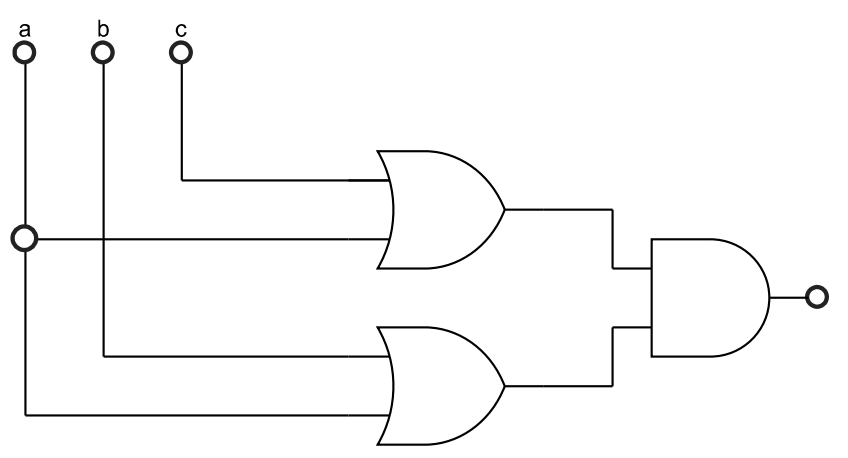
\includegraphics[width=0.9\textwidth]{Circuito2.PNG}
\caption{Circuito resultante de simplificar la expresión (\ref{equ:maxterms}).}
	\label{fig:circ2}
\end{figure}
Luego se dedujo una expresión para escribirlo con compuertas \textbf{NOR}
\[
	f \left( d,c,b,a \right) = \overline{\overline{\bar{a} b c}} + \overline{\overline{a d}} + \overline{\overline{a \bar{c}}} + \overline{\overline{a \bar{b}}}
\]
\[
	f \left( d,c,b,a \right) = \overline{ \left( \bar{a} \ + \ c \right) } \ + \ \overline{ \left( a \ + \ \bar{b} \ + \ \bar{c} \right) } \ + \ \overline{ \left( \bar{a} \ + \ b \right) } \ + \ \overline{ \left( \bar{a} \ + \ \bar{d}\right) }
\]
a la cual le corresponde el siguiente circuito.

\begin{figure}[H]
	\centering
	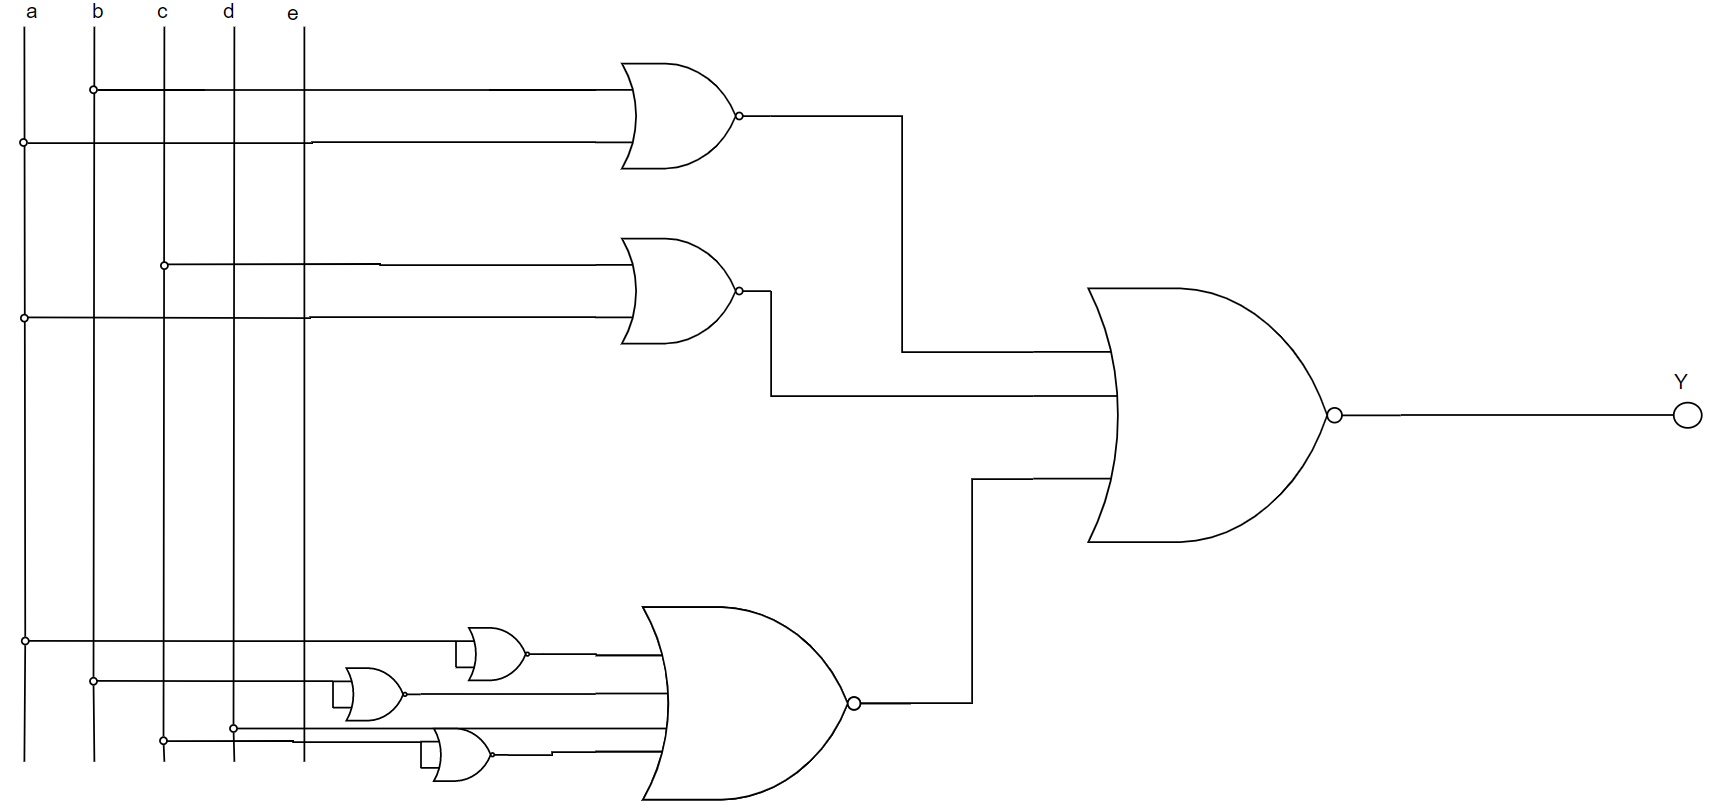
\includegraphics[width=0.9\textwidth]{Circuito5.png}
\caption{Circuito únicamente con compuertas NOR.}
	\label{fig:circ5}
\end{figure}
\subsection*{Ejercicio 3}
En el siguiente ejercicio se procedió a implementar un MUX de 4 entradas y un DECODER de 4 salidas en verilog.
Para realizar dicho MUX se utilizó como entradas un arreglo de 4 bits en el que cada bit corresponde a cada una de las entradas. A su vez se utilizó otro arreglo, pero en este caso de 2 bits donde cada elemento representa los distintos selectores. En este módulo se programó de tal forma que al notarse un cambio en alguna de las entradas o de alguno de los selectores se procede a analizar cuál entrada se debe copiar a la salida.


En lo que corresponde al DECODER de 4 salidas se utilizó un razonamiento análogo pero en este caso se utilizó un arreglo de 2 bits para las 2 entradas y un arreglo de 4 bits para las distintas salidas. Se procedió a analizar según los valores que presentan los dos bits de entrada para así saber que elemento del arreglo de salida había que colocar en 0 o en 1.

\subsection*{Ejercicio 4}
En este punto se pidió armar un circuito que dados 4 bits de entrada en binario, sean transformados a su equivalente en código de Gray. Se armó la tabla de verdad: 
\begin{table}[H]
\centering
\begin{tabular}{|c|c|c|c|c|c|c|c|c|}
\hline
\multicolumn{1}{|c|}{\textbf{$d$}} & \multicolumn{1}{c|}{\textbf{$c$}} & \multicolumn{1}{c|}{\textbf{$b$}} & \textbf{$a$} & \textbf{$m_{ij}$} & \multicolumn{1}{c|}{\textbf{$y_4$}} & \multicolumn{1}{c|}{\textbf{$y_3$}} & \multicolumn{1}{c|}{\textbf{$y_2$}} & \multicolumn{1}{c|}{\textbf{$y_1$}} \\ \hline
0                                  & 0                                 & 0                                 & 0            & \textbf{$m_{i0}$} & 0                                   & 0                                   & 0                                   & 0                                   \\ \cline{5-5}
0                                  & 0                                 & 0                                 & 1            & \textbf{$m_{i1}$} & 0                                   & 0                                   & 0                                   & 1                                   \\ \cline{5-5}
0                                  & 0                                 & 1                                 & 0            & \textbf{$m_{i2}$} & 0                                   & 0                                   & 1                                   & 1                                   \\ \cline{5-5}
0                                  & 0                                 & 1                                 & 1            & \textbf{$m_{i3}$} & 0                                   & 0                                   & 1                                   & 0                                   \\ \cline{5-5}
0                                  & 1                                 & 0                                 & 0            & \textbf{$m_{i4}$} & 0                                   & 1                                   & 1                                   & 0                                   \\ \cline{5-5}
0                                  & 1                                 & 0                                 & 1            & \textbf{$m_{i5}$} & 0                                   & 1                                   & 1                                   & 1                                   \\ \cline{5-5}
0                                  & 1                                 & 1                                 & 0            & \textbf{$m_{i6}$} & 0                                   & 1                                   & 0                                   & 1                                   \\ \cline{5-5}
0                                  & 1                                 & 1                                 & 1            & \textbf{$m_{i7}$} & 0                                   & 1                                   & 0                                   & 0                                   \\ \cline{5-5}
1                                  & 0                                 & 0                                 & 0            & \textbf{$m_{i8}$} & 1                                   & 1                                   & 0                                   & 0                                   \\ \cline{5-5}
1                                  & 0                                 & 0                                 & 1            & \textbf{$m_{i9}$} & 1                                   & 1                                   & 0                                   & 1                                   \\ \cline{5-5}
1                                  & 0                                 & 1                                 & 0            & \textbf{$m_{iA}$} & 1                                   & 1                                   & 1                                   & 1                                   \\ \cline{5-5}
1                                  & 0                                 & 1                                 & 1            & \textbf{$m_{iB}$} & 1                                   & 1                                   & 1                                   & 0                                   \\ \cline{5-5}
1                                  & 1                                 & 0                                 & 0            & \textbf{$m_{iC}$} & 1                                   & 0                                   & 1                                   & 0                                   \\ \cline{5-5}
1                                  & 1                                 & 0                                 & 1            & \textbf{$m_{iD}$} & 1                                   & 0                                   & 1                                   & 1                                   \\ \cline{5-5}
1                                  & 1                                 & 1                                 & 0            & \textbf{$m_{iE}$} & 1                                   & 0                                   & 0                                   & 1                                   \\ \cline{5-5}
1                                  & 1                                 & 1                                 & 1            & \textbf{$m_{iF}$} & 1                                   & 0                                   & 0                                   & 0                                   \\ \cline{5-5}
\hline
\end{tabular}
\end{table}

Se procedió a escribir cada bit de salida en función de los mintérminos:
\[
	y_4 = \sum_{j=8}^{F} m_{4j}  \  ; \ y_3 = \sum_{j=4}^{B} m_{3j}\  ; \ y_2 = \sum_{j=2}^{5} m_{2j} \ + \  \sum_{j=A}^{D} m_{2j}  \  ;\]
\[
	y_1=m_{11}+m_{12}+m_{15}+m_{16}+m_{19}+m_{1A}+m_{1D}+m_{1E} 
\]
luego, para llegar a la forma simplificada, se hizo el mapa de Karnaugh de cada salida:


\begin{centering}
    \begin{Karnaugh}
        \minterms{8,9,10,11,12,13,14,15}
        \maxterms{0,1,2,3,4,5,6,7}
        
        \implicant{12}{10}{red}
   
    \end{Karnaugh}
\par\end{centering}


\begin{table}[H]
\centering
\caption{Mapa de Karnaugh del bit y4 de salida.}
\label{tabla:maxterms}
\end{table}
Se puede ver que $y_4 = d$ del segundo bit:


\begin{centering}
    \begin{Karnaugh}
        \minterms{4,5,6,7,8,9,10,11}
        \maxterms{0,1,2,3,12,13,14,15}
        
        \implicant{4}{6}{red}
        \implicant{8}{10}{red}
    \end{Karnaugh}
\par\end{centering}


\begin{table}[H]
\centering
\caption{Mapa de Karnaugh del  bit y3 de salida.}
\label{tabla:maxterms}
\end{table}
De aquí $$y_3 = \bar{d}c+d\bar{c}$$
continuando para la siguiente salida:


\begin{centering}
    \begin{Karnaugh}
        \minterms{2,3,4,5,10,11,12,13}
        \maxterms{0,1,6,7,8,9,14,15}
        
        \implicant{4}{13}{red}
\implicantdaltbaix[3pt]{3}{10}{red}
    \end{Karnaugh}
\par\end{centering}


\begin{table}[H]
\centering
\caption{Mapa de Karnaugh del bit y2 de salida.}
\label{tabla:maxterms}
\end{table}
De aquí $$y_2 = \bar{c}b+c\bar{b}$$
continuando para la ultima salida:


\begin{centering}
    \begin{Karnaugh}
        \minterms{1,2,5,6,9,10,13,14}
        \maxterms{0,3,4,7,8,11,12,15}        
        \implicant{1}{9}{red}
        \implicant{2}{10}{red}
    \end{Karnaugh}
\par\end{centering}


\begin{table}[H]
\centering
\caption{Mapa de Karnaugh del  bit y1 de salida.}
\label{tabla:maxterms}
\end{table}
Finalmente se obtiene: $$y_1 = \bar{b}a+\bar{a}b$$
Luego se armo el circuito únicamente utilizando compuertas \textbf{OR}, \textbf{AND} y \textbf{NOT}

\begin{figure}[H]
	\centering
	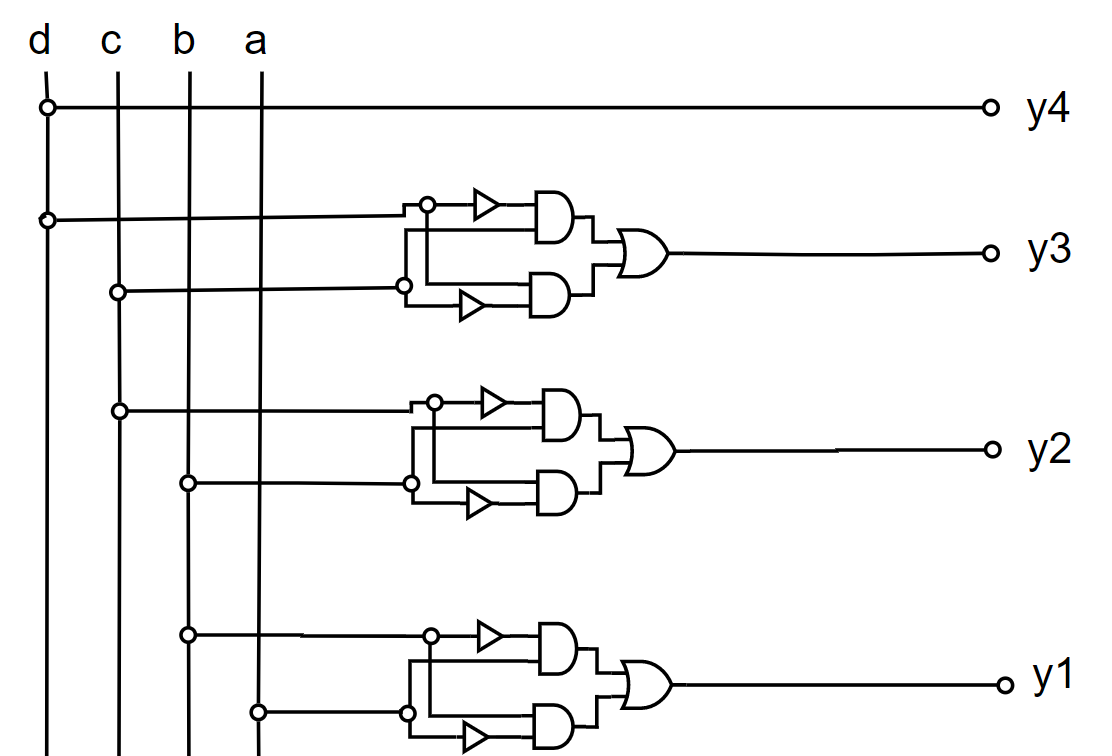
\includegraphics[width=0.9\textwidth]{Circuito3.png}
	\caption{Conversor codigo de Gray.}
	\label{fig:circ3}
\end{figure}
Finalmente, se implementó en verilog un módulo que realiza la conversión de binario a código de gray utilizando la configuración de compuertas de la (\ref{fig:circ3}),
y una test bench que prueba todos los casos posibles.


\subsection*{Ejercicio 5}

En este punto se implementa un modulo en verilog, que reciba dos números en formato \textbf{BCD} y devuelva su producto como dos números en el mismo formato. Se implementó aprovchando el operador de modulo proporcionado por verilog.  Si bien este fue la implementación final inicialmente se habia implementado con un algoritmo el cual consistia en shiftear el numero y en algunos casos sumarle a un nybble en particular 3. Este modelo fue descartado dado a que cuando fue implemetnado se utilizaron ciclos \textbf{for}  lo cual en el lenguaje verilog es muy ineficiente.
A lo largo del la implementación, se presentaron diversas complicaciones, como por ejemplo, determinar el scope que poseen las variables, que bloques dentro de un modulo pueden tomar un set de lineas de manera procedural y como relacionar un modulo con otro.
Luego de haber implementado el código, se procedió a realizar un test-bench, el cual prueba todos los casos posibles que puedan ser recibidos como input por el modulo.


\end{document}

